\documentclass[a4paper, 12pt]{article}
\usepackage[utf8]{inputenc}
\usepackage[italian]{babel}
\usepackage[T1]{fontenc}
\usepackage[hidelinks]{hyperref}
\usepackage{graphicx}

\title{La banca del tempo}
\author{Simone Pozzebon}
\date{March 2021}

\begin{document}

\maketitle
\newpage
\tableofcontents
\newpage

\section{Testo}
\begin{center}
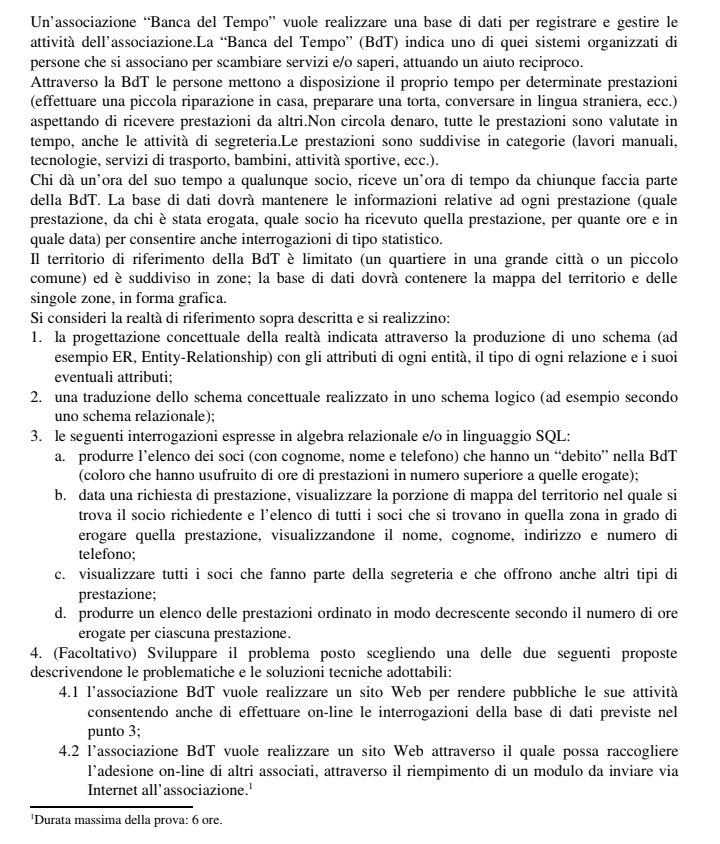
\includegraphics[scale=0.5]{img/testo.png}
\end{center}
\newpage

\section{Analisi}

\subsection{Entit\'a}
\begin{itemize}
    \item \textit{Categoria}, indica le differenti variet\'a di prestazione;
    \item \textit{Prestazione}, indica l'azione effettuata o richiesta da un socio;
    \item \textit{Socio}, individuo delegato per lo svolgimento di una prestazione o richiedente della stessa;
    \item \textit{Zona}, suddivisione delle aree di interesse per lo svolgimento e la richiesta delle prestazioni.
\end{itemize}

\subsection{Diagramma ER}
\begin{center}
\bigskip
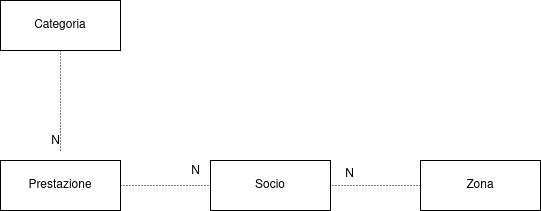
\includegraphics[scale=0.5]{img/er.png}    
\end{center}
\medskip
\begin{itemize}
    \item Per ogni \textit{categoria} pu\'o essere definita una \textit{prestazione}.\\Data una \textit{prestazione} deve esserci una e una soltanto \textit{categoria};
    \item Ogni \textit{socio} pu\'o offrire o richiedere una o pi\'u \textit{prestazioni}. \\
    Ogni \textit{prestazione} pu\'o essere offerta o richiesta da un \textit{socio};
    \item Ogni \textit{socio} risiede in una sola \textit{zona}. \\ Per ogni \textit{zona} possono esserci differenti \textit{soci}.
\end{itemize}
\newpage

\subsection{Attributi}
\begin{itemize}
    \item \textit{Categoria} 
        \begin{itemize}
            \item Id Categoria
            \item Descrizione
        \end{itemize}
    \item \textit{Prestazione} 
        \begin{itemize}
            \item Id Prestazione
            \item Descrizione
            \item Categoria
            \item Data Svolgimento
            \item Data Richiesta
            \item Ora Svolgimento
            \item Socio Richidente
            \item Socio Erogante
        \end{itemize}
    \item \textit{Socio} 
        \begin{itemize}
            \item Id Socio
            \item Nome
            \item Cognome
            \item Cellulare
            \item Mail
            \item Ore Erogate
            \item Ore Richieste
            \item Indirizzo
            \item Zona Di Riferimento
        \end{itemize}
    \item \textit{Zona} 
        \begin{itemize}
            \item Id Zona
            \item Citt\'a
            \item CAP
        \end{itemize}
\end{itemize}

\subsection{Schema Logico}
\begin{itemize}
    \item categorie(\textit{idCategoria}, descCategoria);
    \item prestazioni(\textit{idPrestazione}, descPrest, \underline{categoria},  dataSvolg, dataRich, \underline{socioSvolg}, \underline{socioRich});
    \item socio(\textit{idSocio}, nome, cognome, cellulare, mail, oreSvolg, oreRich, indirizzo, \underline{zona});
    \item zone(\textit{idZona}, citt\'a, cap);
\end{itemize}

\subsection{Query SQL}
\begin{enumerate}
    \item [a.] \textit{produrre l’elenco dei soci (con cognome, nome e telefono) che hanno un “debito” nella BdT
(coloro che hanno usufruito di ore di prestazioni in numero superiore a quelle erogate);}
    \begin{verbatim}
        SELECT cognome, nome, telefono
        FROM soci
        WHERE oreRich > oreSvolg;
    \end{verbatim}
    \item [b.] \textit{data una richiesta di prestazione, visualizzare la porzione di mappa del territorio nel quale si
trova il socio richiedente e l’elenco di tutti i soci che si trovano in quella zona in grado di
erogare quella prestazione, visualizzandone il nome, cognome, indirizzo e numero di
telefono;}
    \begin{verbatim}
        SELECT nome as "Socio Richiedente" ,
        descPrest as "Descrizione Prestazione",  
        zone.citta as "Zona Socio Richiedente", nome, cognome, cellulare 
            FROM soci, zone, prestazioni
            WHERE descPrest = (SELECT descPrest FROM
            soci, prestazioni 
            idSocio=socioRichiedente)
    \end{verbatim}
\end{enumerate}

\end{document}
